%!TEX root = ../Main.tex

% ---------------------------------------------------------
\section{Streams and Flows}
\label{s:Streams}
A \emph{stream} is an array of elements where the indexing dimension is time. As each element is read from the stream it is available only in that moment, and if the consumer wants to re-use the element at a later time it must save it itself. A \emph{flow} is a bundle of related streams, where each stream carries data from a single partition of a larger data set --- we might create a flow consisting of 8 streams where each one carries data from a 1GB partition of a 8GB data set. We manipulate flow endpoints rather than the flows themselves, using the following data types:

\begin{code}
data Sources i m e 
   = Sources
   { arity :: i
   , pull  :: i -> (e -> m ()) -> m () -> m () }

data Sinks   i m e 
   = Sinks   
   { arity :: i
   , push  :: i -> e -> m ()
   , eject :: i -> m () }
\end{code}

Type @Sources i m e@ classifies flow sources which produce elements of type @e@, using some monad @m@, where the streams in the bundle are indexed by values of type @i@. The index type @i@ is typically @Int@ for a bundle of many streams, and @()@ for a bundle of a single stream. Likewise @Sinks i m e@ classifies flow sinks which consume elements of type @e@.

In the @Sources@ type, field @arity@ stores the number of individual streams in the bundle. To receive data from a flow producer we apply the function in the @pull@ field, passing the index of type @i@ for the desired stream, an \emph{eat} function of type @(e -> m ())@ to consume an element if one is available, and an \emph{eject} computation of type @(m ())@ which will be invoked when no more elements will ever be available for that stream. The pull function will then perform its @(m ())@ computation, for example reading a file, before calling our eat or eject, depending on whether data is available.

In the @Sinks@ type, field @arity@ stores the number of individual streams as before. To send data to a flow consumer we apply the @push@ function, passing the stream index of type @i@, and the element of type @e@. The @push@ function will perform its @(m ())@ computation to consume the provided element. If no more data is available we instead call the @eject@ function, passing the stream index of type @i@, and this function will perform an @(m ())@ computation to shut down the sink --- possibly closing files or disconnecting sockets.

Consuming data from a @Sources@ and producing data to a @Sinks@ is synchronous, meaning that the computation will block until an element is produced or no more elements are available (when consuming); or an element is consumed or the endpoint is shut down (when producing). The @eject@ functions used in both @Sources@ and @Sinks@ are associated with a single stream only, so if our flow consists of 8 streams attached to 8 separate files then ejecting a single stream will close a single file.


% ---------------------------------------------------------
\subsection{Sourcing, Sinking and Draining}
Figure~\ref{f:Draining} gives the definitions of @sourceFs@, @sinkFs@ which create flow sources and sinks based on a list of files, as well as @drainP@ which pulls data from a flow source and pushes it to a sink. We elide type class constraints to save space.

Given the definition of the @Sources@ and @Sinks@ types, writing @sourceFs@ and @sinkFs@ is straightforward. In @sourceFs@ we first open all the provided files, yielding file handles for each one, and the @pull@ function for each stream source reads data from the corresponding file handle. When we reach the end of a file we eject the corresponding stream. In @sinkFs@, the @push@ function writes the provided element to the corresponding file, and @eject@ closes it.

The @drainP@ function takes a bundle of stream @Sources@, a bundle of stream @Sinks@, and drains all the data from each source into the corresponding sink. Importantly, @drainP@ forks a separate thread to drain each stream, making the system data parallel. We use Haskell MVars for communication between threads. After forking the workers, the main thread waits until they are all finished. Now that we have the @drainP@ function, we can write the ``hello world'' of data parallel data flow programming: copy a partitioned data set from one set of files to another:

\begin{code}
 copySetP :: [FilePath] -> [FilePath] -> IO ()
 copySetP srcs dsts
  = do  ss <- sourceFs srcs
        sk <- sinkFs   dsts
        drainP ss sk
\end{code}

% In our concrete implementation we also include a @drainS@ (sequential) which evaluates each stream in turn rather than concurrently.
%% trying to remove space, do not think this is necessary

\begin{figure}
\begin{code}
sourceFs :: [FilePath] -> IO (Sources Int IO Char)
sourceFs names 
 = do hs <- mapM (\n -> openFile n ReadMode) names
      let pulls i ieat ieject
          = do let h = hs !! i
               eof <- hIsEOF h
               if eof then hClose   h >> ieject
                      else hGetChar h >>= ieat
      return (Sources (length names) pulls)

sinkFs  :: [FilePath] -> IO (Sinks Int IO Char)
sinkFs names 
 = do hs <- mapM (\n -> openFile n WriteMode) names
      let pushs  i e = hPutChar (hs !! i) e
      let ejects i   = hClose   (hs !! i)
      return (Sinks (length names) pushs ejects)

drainP :: Sources i IO a -> Sinks i IO a -> IO ()
drainP (Sources i1 ipull) (Sinks i2 opush oeject)
 = do mvs <- mapM makeDrainer [0 .. min i1 i2]
      mapM_ readMVar mvs
 where
  makeDrainer i = do
    mv <- newEmptyMVar
    forkFinally (newIORef True >>= drainStream i)
                (\_ -> putMVar mv ())
    return mv
  drainStream i loop =
    let eats v = opush i v
        ejects = oeject i >> writeIORef loop False
    in  while (readIORef loop) (ipull i eats ejects)
\end{code}
% This was the best I could do with the updated drainP function.
% I think the 'while' function is obvious enough to not be defined.

\caption{Sourcing, Sinking and Draining}
\label{f:Draining}
\end{figure}


% ---------------------------------------------------------
\subsection{Stateful Streams, Branching and Linearity}
\label{s:Linearity}
Suppose we wish to copy our files while counting the number of characters copied.
To count characters we can @map@ each to the constant integer one, then perform a @fold@ to add up all the integers. To avoid reading the input data from the file system twice we use a counting process that does not force the evaluation of this input data itself. For this reason we use versions of @map@ and @fold@ that produce new @Sinks@ rather than @Sources@. Their types are as follows:
\begin{code}
map_o  :: (a -> b) -> Sinks i m b -> Sinks i m a

fold_o :: Ord i => i -> (a -> a -> a) -> a
                -> IO (Sinks i IO a, IORef a)
\end{code}
The @map_o@ operator transforms a sink of @b@ things into a sink of @a@ things. The @fold_o@ operator produces a sink for @a@ things, and an @IORef@. The value in the @IORef@ is initialised to the given starting value of type @a@, which is combined with elements pushed to the sink using the worker function of type @(a -> a -> a)@. The first argument of type @i@ is the arity of the result sinks. 

Besides @map_o@ and @fold_o@ we also need an operator to branch the flow so that the same data can be passed to our counting operators as well as written back to the file system. 

\eject
The branching operator we use is as follows:

\begin{code}
dup_ooo :: (Ord i, Monad m)
       => Sinks i m a -> Sinks i m a -> Sinks i m a
dup_ooo (Sinks n1 push1 eject1) 
        (Sinks n2 push2 eject2)
 = let pushs  i x = push1 i x >> push2 i x
       ejects i   = eject1 i  >> eject2 i
   in  Sinks (min n1 n2) pushs ejects
\end{code}

This operator takes two argument sinks and creates a new one. When we push an element to the new sink it will push that element to the two argument sinks. Likewise, when we eject a stream in the new sink it will eject the corresponding stream in the two argument sinks. We can use this new combinator to write a working @copyCountP@ function:

\begin{code}
copyCountP :: [FilePath] -> [FilePath] -> IO Int
copyCountP srcs dsts
 = do  ss      <- sourceFs srcs
       sk1     <- sinkFs   dsts
       (sk2,r) <- fold_o  (arity ss) (+) 0 
       drainP ss (dup_oo sk1 (map_o (const 1) sk2))
       readIORef r
\end{code}

This function runs in constant space, using a single pass over the input data, which is the behaviour we wanted. Note that in the definition there is only a single occurrence of each of the variables bound to sources and sinks: @ss@, @sk1@, @sk2@. Each source and sink is used linearly. Our program expresses a data flow graph where the functions @sourceFs@, @sinkFs@, @fold_o@, @map_o@ and @dup_ooo@ create nodes, and the use-def relation of variables defines the edges.

\eject
Linearity is an important point. Suppose we instead tried to compute our result in two separate stages, one to copy the files to their new locations and one to compute the count:
\begin{code}
badCopyCount :: [FilePath] -> [FilePath] -> IO Int
badCopyCount srcs dsts
 = do  ss      <- sourceFs srcs
       sk1     <- sinksFs  dsts
       drainP ss sk1
       (sk2,r) <- fold_o (+) 0 (arity ss)
       drainP ss (map_o (const 1) sk2)
       readIORef r
\end{code}

This cannot work. The @Sinks@ endpoint created by @sourceFs@ is a stateful object -- it represents the current position in each of the source files being read. After we have applied the first @drainP@, we have already finished reading through all the source files, so draining the associated flow again does not yield more data. In general an object of type @Sources@ is an abstract producer of data, and it may not even be possible to rewind it to a previous state --- suppose it was connected to a stream of sensor readings. Alas the Haskell type system does not check linearity so we rely on the programmer to enforce it manually.


% ---------------------------------------------------------
\subsection{Polarity and buffering}
\label{s:Polarity}
Our @dup_ooo@ operator from the previous section branches a flow by taking two existing sinks and producing a new one. The @_ooo@ suffix stands for ``output, output, output'', referring to the three sinks. It turns out that the converse @dup_iii@ operator is not implementable without requiring unbounded buffering. Such an operator would have the following type:
\begin{code}
 dup_iii :: (Ord i, Monad m)
         =>  Sources i m a 
         -> (Sources i m a, Source i m a)
\end{code}

Consider how this would work. The @dup_iii@ operator takes an argument source and produces two result sources. Now suppose we pull data from the left result source. The operator would need to pull from its argument source to retrieve the data, then when we pull from the right result source we want this same data. The problem is that there is nothing stopping us from pulling the entire stream via the left result source before pulling any elements from the right result source, so @dup_iii@ would need to introduce an unbounded buffer to store all elements in the interim.

Interestingly, although @dup_iii@ cannot work without an unbounded buffer, a hybrid operator @dup_ioi@ can. This operator has the following definition:
\begin{code}
dup_ioi :: (Ord i, Monad m)
        => Sources i m a -> Sinks i m a 
        -> Sources i m a
dup_ioi (Sources n1 pull1) (Sinks n2 push2 eject2)
 = let pull3 i eat3 eject3
        = pull1 i eat1 eject1
        where eat1 x = eat3 x >> push2  i x
              eject1 = eject3 >> eject2 i
   in  Sources (min n1 n2) pull3
\end{code}

The @dup_ioi@ operator takes an argument source, an argument sink, and returns a result source. When we pull data from the result the operator pulls from its argument source and then \emph{pushes} the same data to the argument sink. Similarly to @dup_ooo@, we can use @dup_ioi@ to introduce a branch into the data flow graph \emph{without} requiring unbounded buffering of the input flow. This fact was also noticed in~\cite{Bernardy:Duality}.

\eject
We can extend @dup_iooi@ to work with any number of argument sinks, for example:
\begin{code}
 dup_iooi
  :: (Ord i, Monad m)
  => Sources i m a -> Sinks i m a -> Sinks i m a
  -> Sources i m a
\end{code}

With @dup_ioi@ when we pull from the result source the operator pulls from its argument source and pushes the same data to its argument sinks. 

Figure~\ref{f:Polarity} shows the possible \emph{polarity versions} for the flow duplication operator. Sources are indicated with a $\bullet$ and sinks with a $\circ$. We use the mnemonic that the filled $\bullet$ can always produce data (being a source) while the empty $\circ$ can always accept data (being a sink). In the figure the versions in red would require unbounded buffering, while the black ones require no buffering.

\begin{figure}
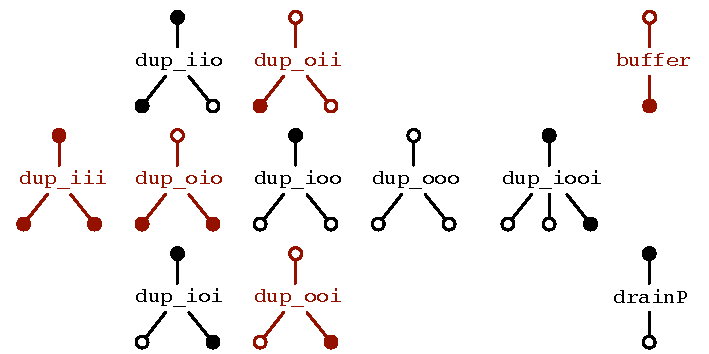
\includegraphics[scale=0.7]{figures/polarity.pdf}

\caption{Possible polarities for the flow duplication operator}
\label{f:Polarity}
\end{figure}

In the right of Figure~\ref{f:Polarity} we have also included the corresponding diagrams for the @drainP@ operator from Figure~\ref{f:Draining}. The @drainP@ operator requires no buffering because all data pulled from the source is immediately pushed to the sink. On the other hand, if we invert the polarities of @drainP@ we arrive at the natural assignment for a primitive buffering operator. Any operator that accepts data via a single argument sink and produces the same data via a result source \emph{must} introduce a buffer, as there is no guarantee that new elements are pushed to the sink at the same rate they are pulled from the source. Our Repa Flow library guarantees that programs written with it run in constant space by only providing operators in the polarity versions that do so.


% ---------------------------------------------------------
\subsection{Mapping}
\label{s:Mapping}
We mentioned the @map_o@ operator back in \S\ref{s:Linearity}. Here is its type again, along with the matching @map_i@ with inverse polarity:

\begin{code}
map_o :: (a -> b) -> Sinks   i m b -> Sinks   i m a
map_i :: (a -> b) -> Sources i m a -> Sources i m b
\end{code}

\begin{figure}
\begin{center}
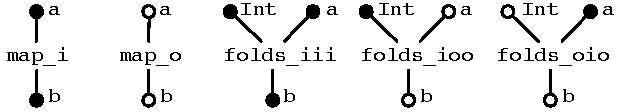
\includegraphics[scale=0.8]{figures/maps.pdf}
\end{center}
\vspace{-0.5em}
\caption{Polarities for \texttt{map} and \texttt{folds}}
\label{f:Map}
\end{figure}

The first form is a sink transformer, taking a sink of elements of type @b@ and returning a sink of elements of type @a@. The second is a source transformer, taking a source of elements of type @a@ and returning a source of elements of type @b@. The polarity diagram for both forms is given in Figure~\ref{f:Map}. In both cases the input elements have type @a@ and the output elements have type @b@. The definition of @map_i@ is as follows:
\begin{code}
map_i :: (a -> b) -> Sources i m a -> Sources i m b
map_i f (Sources n pullsA)
 = Sources n pullsB
 where  pullsB i eatB ejectB
         = pullsA i eatA ejectA
         where  eatA v = eatB (f v)
                ejectA = ejectB
\end{code}

% We have written this definition using separate let-bindings for each intermediate function, rather than with a single inline lambda abstraction for two reasons:
% \begin{enumerate}
% \item When writing larger functions using contination passing style we begin to feel worringly inside-out. Using intermediate bindings allows us to name each function with the type it expects, which makes the code easier to follow.
% \item It allows us to attach INLINE pragmas to each bound name. This is a critical part of our fusion system, which we will discuss further in \S\ref{s:Chunked}.
% \end{enumerate}

Note that both @map_i@ and @map_o@ are simply flow transformers, and are neither inherently parallel or sequential. Repa Flow provides data parallelism, and this parallelism is introduced by the singular @drainP@ function. In this respect @drainP@ is similar to the @computeP@ function over delayed arrays from our original Repa library \cite{Lippmeier:Guiding}, except that parallelism is introduced on a per-stream level rather than a per-element level. We will return to the definition of @map_i@ when we discuss chunking in \S\ref{s:Chunked}.


% ---------------------------------------------------------
\subsection{Segmented Folding}
Figure~\ref{f:Map} includes polarity diagrams for three forms of segmented fold. The first one, @folds_iii@ has the following type:
\begin{code}
folds_iii :: (Ord i, Monad m) => (b -> a -> b) -> b
          -> Sources i m Int  -> Sources i m a 
          -> Sources i m b
\end{code}

The @folds_iii@ operator takes a flow of segment lengths, a flow of elements, and uses the provided combining function and neutral value to fold segments from each stream in the flow. For example, suppose we have the following flows, writing the streams of elements in each flow using nested list syntax:
\begin{code}
folds_iii (+) 0 
   [ [3     2   1] [2   2  ] [4      ] ] 
   [ [1 2 3 1 1 5] [3 3 4 4] [4 3 2 1] ]
 = [ [6     2   5] [6   8  ] [10     ] ]
\end{code}

For the first stream the segment lengths are @[3 2 1]@ and the elements are @[1 2 3 1 1 5]@, we sum up the first three elements, then the next two, then the next one, yielding @[6 2 5]@ for that stream. When @drainP@ from Figure~\ref{f:Draining} is applied to the result source, each of the individual streams in the flow is folded in parallel. 

With @folds_iii@ we assume that both the segment lengths and elements are available as sources. When this is true, evaluation of @folds_iii@ requires no buffering. When we pull a fold result from the result source, the operator pulls the segment length from its argument source, then the corresponding elements from the element source, folding them in the process. 

As per Figure~\ref{f:Map} we can assign polarities to @folds@ in two other ways that allow the operator to execute without buffering. 

With @folds_ioo@ we push elements to the element sink (on the right). As needed, the operator pulls segment lengths from the segment length source (on the left), which instruct it how many of the consecutive elements to fold. As each segment is completed it pushes the result to the result sink (on the bottom).

With @folds_oio@ we push segment lengths to the segment length sink (on the left). As needed, the combinator pulls the corresponding number of elements from the element source (on the right) and folds them. As each segment is completed it pushes the result to the result sink (on the bottom). 

One might wonder if @folds_iii@, @folds_ioo@ and @folds_oio@ are the only versions that can execute without buffering. There are a total of 8 polarity versions for a 3-leg operator such as @folds@.

\eject
Case analysis reveals that the others require unbounded buffering, except for the following special version:
\begin{center}
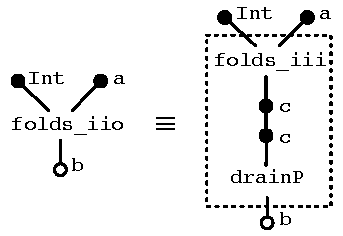
\includegraphics[scale=0.8]{figures/folds-drain.pdf}
\end{center}

The @folds_iio@ version does not require buffering because all segment lengths and elements are available as sources, and the result of folding each segment can be pushed directly to the result sink. However, this version is not primitive as it can be expressed as the composition of @folds_iii@ and @drainP@ as shown above. We refer to a polarity version that can be expressed as a composition with @drainP@ as an \emph{active version}, because its form implies computation rather than being an \emph{inactive} transformation on sources on sinks. Note that @dup_ioo@ from Figure~\ref{f:Polarity} is also active.

In our Repa Flow library we provide only polarity versions that execute without buffering, and the only active versions are @drainP@ and @drainS@ (sequential drain). This restriction ensures that it is easy for the programmer to reason about when computation happens, as well as having the programs execute in constant space.


% ---------------------------------------------------------
\subsection{Stream projection, funneling, and fattening}
So far the operators we have discussed have all performed the same computation each stream in the flow. Here are four basic operators to convert between flows consisting of several streams and \emph{singleton} flows, containing only one stream. The endpoints for singleton flows have the index type set to @()@ which indicates there is only one stream in the flow.
\begin{code}
project_i :: i -> Sources i m a -> Sources () m a
project_o :: i -> Sinks   i m a -> Sinks   () m a

funnel_i :: Sources i IO a ->  IO (Sources () IO a)
funnel_o :: i -> Sinks () IO a -> IO (Sinks i IO a)
\end{code}
% the extra index argument to funnel_o messes up layout, and it's such a small implementation detail that I don't think it's worth putting in.

The @project@ operators each take a stream index, an endpoint for a flow of several streams, and return an endpoint for a singleton flow containing only the specified stream. The @project_i@ operator takes a flow source of several streams, and returns a flow source that selects only the specified stream. The @project_o@ operator takes a flow sink for several streams and returns a sink that discards data in all streams except the specified one.

The @funnel@ operators each take an endpoint for a flow of several streams, and return a singleton flow containing \emph{all} data in the argument flow. The @funnel_o@ opeartor also takes the desired arity of the result @Sinks@. These operators expose a duality in the inversion of control associated with a stream combinator library:

With @funnel_i@ the order in which the argument streams are processed is under the control of the \emph{operator} and is \emph{deterministic} when viewed by the consumer of the result source. In our implementation the default order is to send data from each argument stream from lowest index to highest. Other orders are possible, such as a round-robin process that produces a single element from each non-empty stream in turn. 

In contrast, with @funnel_o@ the order in which argument streams are processed is controlled by the \emph{context} and is \emph{non-deterministic} when viewed by the consumer attached to the argument sink. Recall that in the implementation of @drainP@ from Figure~\ref{f:Draining} we forked a thread to evaluate each source stream. As each of these threads pushes to its corresponding sink concurrently, if these sinks are then funneled then the order in which elements appear in the output may vary from run to run. As the sink may be attached to a shared resource such as a file, this is also the place in the library where we must introduce locks to manage contention. Other operators such as @map@ and @folds@ are lock free, as although they are applied to flow endpoints that conceptually carry several streams at once, at runtime there is no communication between the threads that evaluate each of these streams.

The fact that @funnel_o@ is more complex to implement than @funnel_i@ stems from the ``central dogma'' of data flow programming: information flows from inputs to outputs. If it also flowed the other way then @funnel_i@ would also need locks. The central dogma suggests a natural program transformation, which we name \emph{drain fattening}:
\begin{alltt}
    (funnel_i           s >>= \(\lambda\)s'. drainP s' k)
 => (funnel_o (arity s) k >>= \(\lambda\)k'. drainP s  k')
\end{alltt}

This is better expressed as a picture:
\begin{center}
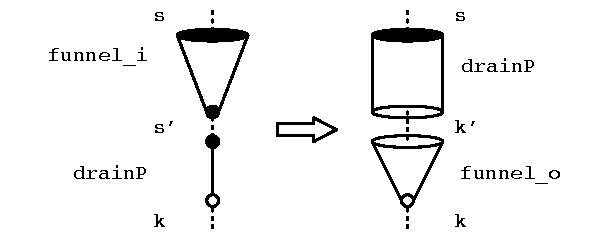
\includegraphics[scale=0.8]{figures/drain-fatten.pdf}
\end{center}

Drain fattening is valid provided the consumer of the final result source @k@ performs a commutative reduction, or is otherwise insensitive to the order in which elements arrive. By exchanging the order of @drainP@ and @funnel@ we allow parallel evaluation of multiple streams in the flow, at the expense of introducing non-determinism in the order in which elements are pushed to the sink. Drain fattening expresses the change in computation structure that arises when moving from a process that performs sequential reduction of a data set, to one that performs parallel tree reduction. However, in our case the change in computation structure is separated from the need to actually perform a reduction.

% In future work it would be interesting to add a phantom type parameter to our @Sinks@ data type to represent the fact that a particular sink is insensitive to the order in which elements arrive. This would enable us to fatten our drains automatically, but for now the transformation must be performed by hand.

Finally, although the syntactic transform requires @funnel_i@ to be close to @drainP@, the fact that our operators come in a variety of polarity versions allows us to pull many through a @drainP@ to bring their arguments closer, for example:
\begin{alltt}
  drainP (map_i f s) k  =  drainP s (map_o f k)
\end{alltt}

